% -*- coding: utf-8 -*-

\chapter{Métodos de trabajo y herramientas}
\label{chap:methods}
\drop{E}{l} siguiente capítulo expone la metodología de trabajo escogida para
llevar a cabo el desarrollo del proyecto y describe las principales 
herramientas utilizadas para llevarlo a cabo.

\section{Pasos previos}
Antes de elegir una metodología concreta, conviene realizar un estudio rápido
de campo, para identificar cuáles son las partes que componen el sistema y para
definir \emph{a grosso modo} cuáles son las necesidades de información.

  \subsection{Estudio de campo}
  \label{sec:fieldStudy}
Como todo el mundo sabe, un restaurante es un \emph{``establecimiento público 
donde se sirven comidas y bebidas, mediante precio, para ser consumidas en el
mismo local''}~\cite{bib:rae}.

Hoy en día existe una gran variedad de tipos de restaurante y de modalidades
de servicios.

    \subsubsection{Tipos de restaurantes}
  En cuanto a los tipos de establecimientos y fórmulas de restauranción, pueden
  distinguirse cinco clases~\cite{bib:wiki}:
  \begin{itemize}
  \item \textbf{Tipo \emph{buffet}}. Los clientes escogen entre una serie de
  platos cocinados y dispuestos para el autoservicio. Normalmente se oferta
  una gran variedad de productos, pensados para todo tipo de clientes (figura
  \ref{fig:buffet}). El precio por comensal suele ser fijo, aunque también
  existe la modalidad de cobrar por peso o por tipo de platos consumidos.

  \begin{figure}[!h]
    \begin{center}
      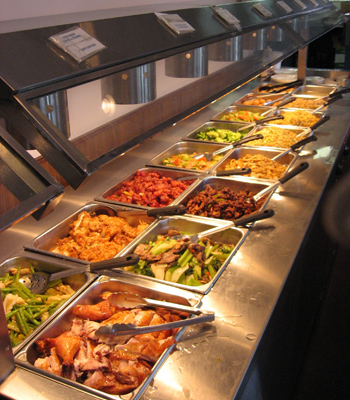
\includegraphics[width=0.5\textwidth]{buffet.png}
      \caption{Restaurante tipo \emph{buffet}.}
      \label{fig:buffet}
    \end{center}
  \end{figure}

  \item \textbf{Tipo \emph{fast food}}. Son restaurantes informales en los que
  se consumen platos de rápida preparación como: hamburguesas, perritos
  calientes, patatas fritas, pizzas o \emph{kebabs}, entre otros (figura
  \ref{fig:fastFood}). El usuarios de estos establecimientos busca la rapidez 
  del servicio, no la calidad nutricional o estética de los alimentos 
  servidos. Son, por lo general, los restaurantes más económicos.

  \begin{figure}[!h]
    \begin{center}
      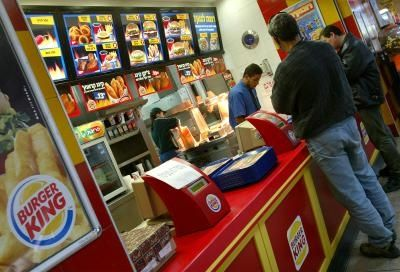
\includegraphics[width=0.6\textwidth]{fastFood.png}
      \caption{Restaurante de comida rápida.}
      \label{fig:fastFood}
    \end{center}
  \end{figure}

  \item \textbf{Tipo \emph{gourmet}}. Son restaurantes de más nivel, tanto por
  los productos preparan, como por la ambientación, la decoración y la atención
  que se ofrece (figura \ref{fig:gourmet}). Los pedidos son ``a la carta'' o
  escogidos de un ``menú'', por lo que los alimentos son cocinados al momento.
  Las mesas son atendidas por una serie de camareros dirigidos por un
  \emph{Maître}. El costo va en relación al servicio recibido y a la calidad de
  los platos consumidos.

  \begin{figure}[!h]
    \begin{center}
      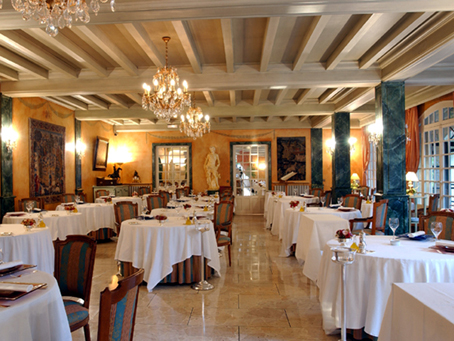
\includegraphics[width=0.7\textwidth]{gourmet.png}
      \caption{Restaurante tipo \emph{gourmet}.}
      \label{fig:gourmet}
    \end{center}
  \end{figure}

  \item \textbf{Tipo temático}. Son restaurantes que sirven exclusivamente
  productos típicos de un país o cultura. Suelen estar decorados y ambientados
  con motivos propios de la zona a la que representan (figura
  \ref{fig:themed}). Los tipos de cocina más populares en todo el mundo son: 
  la cocina italiana o la cocina china. Aunque también están muy extendidos 
  los restaurantes de cocina japonesa, brasileña, turca, india o tailandesa,
  entre otros.

  \begin{figure}[!h]
    \begin{center}
      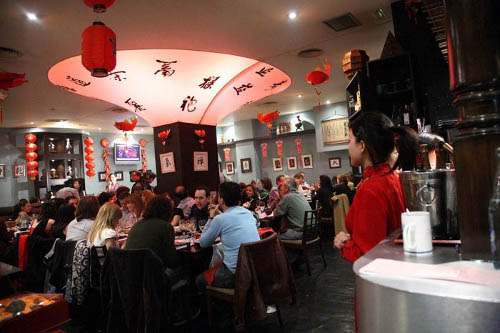
\includegraphics[width=0.7\textwidth]{themed.png}
      \caption{Restaurante con temática china.}
      \label{fig:themed}
    \end{center}
  \end{figure}

  \item \textbf{Tipo \emph{take away}}. Son similares a los restaurantes de
  comida rápida (\emph{fast food}), tanto en la rapidez del servicio, como en 
  el precio y en la calidad de los alimentos. El cliente se confecciona su 
  menú, eligiendo entre una serie de productos expuestos en vitrinas (frías y 
  calientes) (figura \ref{fig:takeAway}) y tiene la opción de consumirlos 
  dentro del establecimiento o puede llevárselos fuera. La vajilla y el menaje 
  que se usan son recipientes desechables.

  \begin{figure}[!h]
    \begin{center}
      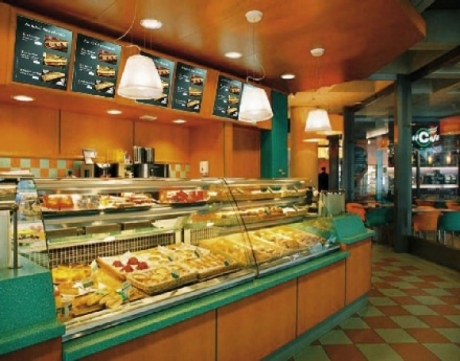
\includegraphics[width=0.6\textwidth]{takeAway.png}
      \caption{Restaurante tipo \emph{take away}.}
      \label{fig:takeAway}
    \end{center}
  \end{figure}

  \end{itemize}

  Las categorías citadas anteriormente no son excluyentes. Es decir, un
  restaurante puede estar clasificado en varias categorías. Por ejemplo, es muy
  común que los restaurantes de comida rápida (\emph{fast food}) ofrecezcan los
  servicios de restaurantes con comida para llevar (\emph{take away}). O los
  restaurantes temáticos pueden ofrecer un servicio tipo \emph{gourmet}.

    \subsubsection{Tipos de servicio}
  Según la forma de preparar, presentar y servir la comida y la bebida, un
  restaurante puede tener~\cite{bib:wiki}:
  \begin{itemize}
  \item \textbf{Servicio francés}. La principal característica de este tipo de
  servicio es que el menú es elaborado en presencia del cliente (figura
  \ref{fig:frenchService}). Es decir, los ingredientes se traen de la cocina y
  se muestran al cliente para su inspección. A continuación, son devueltos a la
  cocina, donde se preparan. Y, una vez cocinados, el \emph{maître} prepara las
  raciones frente a la mesa, a gusto de cada comensal y las va sirviendo 
  siempre por la izquierda. Este tipo de servicio requiere gran habilidad por 
  parte del personal y por tanto resulta bastante caro. Es por ello que, sólo 
  suele emplearse en los restaurantes de más alto nivel.

  \begin{figure}[!h]
    \begin{center}
      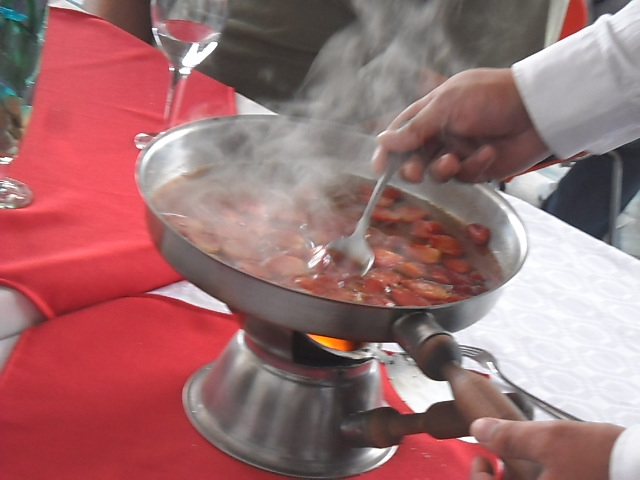
\includegraphics[width=0.6\textwidth]{frenchService.png}
      \caption{\emph{Maître} preparando raciones frente a una mesa. Típico del 
      \emph{servicio francés}.}
      \label{fig:frenchService}
    \end{center}
  \end{figure}

  \item \textbf{Servicio a la rusa}. Al sentarse, cada comensal encuentra 
  frente a él un plato vacío (el plato de servicio), sobre el que hay colocada 
  una servilleta. Y a izquierda y derecha se extienden los cubiertos que va a
  utilizar (salvo los del postre y alguno específico para carne o pescado)
  (figura \ref{fig:russianService}). Tras elegir aquello que va a tomar, se
  retira el plato de servicio y se van trayendo los platos encargados 
  siguiendo un orden específico (usualmente: sopas y entremeses, primeros 
  platos, segundos platos y postres). Cuando un comensal ha acabado con un 
  plato, el camarero lo retira y le trae el siguiente. Los platos son servidos 
  completamente preparados y presentados, por lo que no se requiere una 
  cualificación especial para los camareros. Esto ayuda a economizar y 
  dinamizar el servicio. En este caso, el \emph{maître} sólamente actúa como 
  jefe de sala, no sirve platos. Es el tipo de servicio de restaurantes más 
  extendido.

  \begin{figure}[!h]
    \begin{center}
      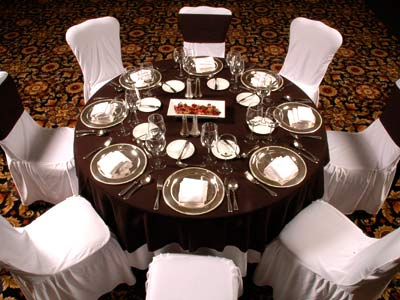
\includegraphics[width=0.6\textwidth]{russianService.png}
      \caption{Mesas equipadas conforme al \emph{servicio a la rusa}.}
      \label{fig:russianService}
    \end{center}
  \end{figure}

  \item \textbf{Servicio a la inglesa}. El comensal encuentra una disposición
  similar a la del \emph{servicio a la rusa}, con la diferencia de que, en este
  caso, el camarero sirve los alimentos desde una fuente o bandeja (siempre por
  la izquierda) (figura \ref{fig:englishService}). Como ocurría en el
  \emph{servicio francés}, el camarero va sirviendo sólamente el producto y la
  cantidad que el cliente solicita. En este tipo de servicio la presentación 
  del plato se pierde y es algo incómodo, tanto para el camarero como para el 
  comensal. Suele emplearse en algunos banquetes.

  \begin{figure}[!h]
    \begin{center}
      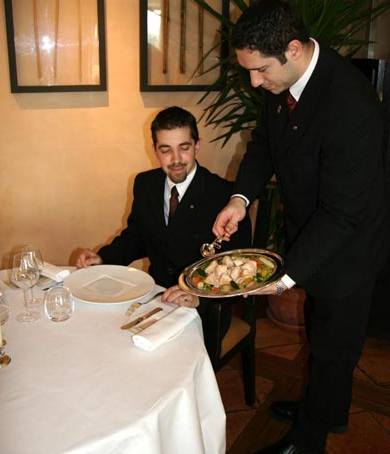
\includegraphics[width=0.4\textwidth]{englishService.png}
      \caption{Camarero sirviendo conforme al \emph{sercicio a la inglesa}.}
      \label{fig:englishService}
    \end{center}
  \end{figure}

  \item \textbf{Servicio americano}. Es una simplificación del \emph{servicio a
  la rusa} en el que se prima la rapidez. Los platos y las bebidas se sirven
  por la derecha y se retiran por la izquierda. Los alimentos que se sirven
  requieren poca preparación, tanto para su elaboración como para su servicio
  (figura \ref{fig:americanService}). Es el tipo de servicio más económico.

  \begin{figure}[!h]
    \begin{center}
      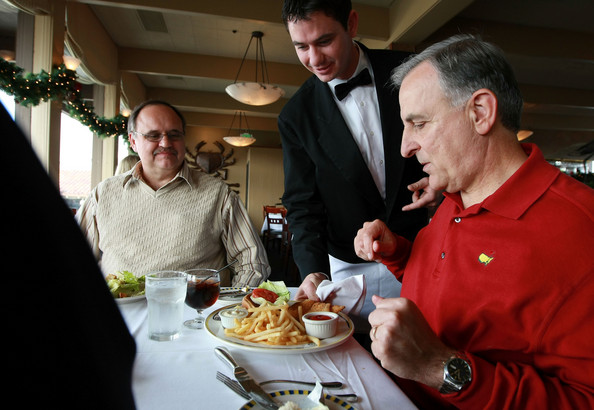
\includegraphics[width=0.6\textwidth]{americanService.png}
      \caption{Camarero sirviendo conforme al \emph{sercicio americano}.}
      \label{fig:americanService}
    \end{center}
  \end{figure}

  \end{itemize}

  Los restaurantes \emph{take away}, \emph{fast food} y \emph{buffet} suelen
  carecer de camareros y, por lo tanto, no pueden englobarse dentro de ninguno 
  de los tipos de servicio nombrados anteriormente. En cuanto a los 
  restaurantes de alta cocina (o \emph{gourmets}) y a los \emph{restaurantes 
  temáticos}, el tipo de servicio ofrecido está directamente relacionado con 
  el nivel del establecimiento.

  \subsection{Consideraciones del escenario}
    \subsubsection{Restaurante tipo}
  El presente \acs{PFC} va - en principio - orientado a restaurantes de tipo
  \emph{gourmet} o \emph{temático}, que son restaurantes que cuentan con
  servicio de camareros y disponen de una carta de productos. Además, el
  restaurante debe contar con un punto de  control de entrada o
  \textbf{recibidor}, que debe estar custodiado por un \emph{maître}. Este se
  encargará de atender a los clientes que entran y les procurará asiento.

  Un trabajo futuro podría consistir en adaptar el sistema para restaurantes 
  de tipo \emph{fast food} o \emph{take away} (que no tienen control de 
  entrada). Para restaurantes tipo \emph{buffet}, en cambio, no tendría
  sentido automatizar los pedidos, puesto que no existen.

  Por otro lado, el tipo de servicio ofrecido no va a afectar al funcionamiento
  del sistema a desarrollar.

    \subsubsection{Necesidades de información}
  En primer lugar, el sistema debe ser capaz de gestionar la información
  típica con la que trabajan la mayor parte de las aplicaciones de
  restauración que existen hoy en día. Es decir, debe gestionar: la lista
  de productos puestos a la venta; el precio, los impuestos y los
  descuentos de cada uno de ellos; el estado, la lista de pedidos y la
  facturación de cada mesa; etc.

  Por otro lado, el sistema está encaminado a que el cliente pueda 
  identificarse a través de su dispositivo móvil, para: realizar
  pedidos desde su mesa, recibir descuentos y recomendaciones según su
  historial y poder realizar pagos mediante \acs{NFC}. Por lo que, otro de los
  objetos a tener en cuenta \textbf{son los clientes} y el historial que dejan
  a través de sus pedidos y accesos al local.

    \subsubsection{Elección de tecnologías}
  El sistema estará formado por varias aplicaciones que se comunican entre sí.
  Para gestionar los datos con los que trabajan las aplicaciones del
  restaurante se contará con una \textbf{base de datos} distribuida, a la que
  se accederá a través de \textbf{servicios web}. Con esto se conseguirá la
  sincronización y la persistencia de los datos con los que se están trabajando
  en cada momento.

  El uso combinado de la \textbf{tecnología \acs{NFC}} con el de las
  \textbf{etiquetas \acs{RFID}}, permitirán al cliente interactuar con los
  elementos del restaurantes, con el simple hecho de acercar su dispositivo
  móvil a una o a otra etiqueta.

  La tecnología móvil inalámbrica que ofrece mayores posibilidades a la hora
  de comunicar el dispositivo móvil con los equipos fijos del restaurante es
  la tecnología \acs{WiFi}. No obstante, el único dispositivo móvil con el que
  se cuenta (\emph{\textbf{Nokia 6131 \acs{NFC}}}, facilitado por el
  \textbf{\emph{grupo \acs{MAmI}\footnote{Grupo de investigación de la
  \acs{UCLM} que tiene como principal objetivo adaptar las tecnologías para 
  modelar contextos en los que se minimice o desaparezca la interacción del 
  usuario de tal manera que éste perciba la asistencia del entorno que le 
  rodea.}}} y que incluye la tecnología \acs{NFC}) no
  dispone esa tecnología. Por ello, se opta por echar mano de otra de las
  tecnologías inalámbricas más extendidas entre los dispositivos móviles, la
  \textbf{tecnología \emph{Bluetooth}}.

  \subsection{Aplicación de los servicios web}
    \subsubsection{Gestión de los datos de un restaurante}
  Como se comentó anteriormente, para garantizar la sincronización de los
datos con los que trabajan las aplicaciones de escritorio del sistema, se va a
definir una aplicación que ofrezca todos los \emph{servicios web} que dichas
aplicaciones necesiten. Es decir, cuando una de estas aplicaciones genere o
necesite algún dato, este será solicitado al \emph{servicio web}
correspondiente.

  Los datos representan el activo más importante del sistema y por ello es
necesario garantizar su integridad. Para conseguirlo, la aplicación que
implementa los \emph{servicios web} será la única que tendrá acceso a una
\emph{base de datos} distribuida donde almacenarán y recuperarán todos los
datos del sistema.

    \subsubsection{Servicios web en \texttt{.NET}}
La aplicación que da cabida a los servicios web va a implementarse utilizando
el \emph{framework} \texttt{.NET}, al igual que las dos aplicaciones de
escritorio.

Para el desarrollo de servicios web en \texttt{.NET} es conveniente hacer uso
del \acs{IDE} estándar de dicho \emph{framework}, es decir, de \texttt{Visual
Studio}:
\begin{enumerate}
\item En primer lugar, se creará un nuevo proyecto \texttt{C\#} del tipo
``\texttt{ASP .NET Web Service}''.
\item A continuación, se añadirá al proyecto un nuevo servicio web. Los
servicios web aparecen en el proyecto como un archivo con extensión
``\texttt{.asmx}''.
\item En el código del fichero ``\texttt{.asmx}'' que se acaba de crear, se
añadirá el atributo \texttt{WebService} para indicar el
\emph{namespace}\footnote{Es una palabra clave de \texttt{.NET} que se utiliza
para declarar un \emph{ámbito}. Este \emph{ámbito} permite organizar el código
y proporciona una forma de crear tipos globalmente únicos. Un mismo
\emph{namespace} puede dar cabida a varios proyectos.} al que pertenecerá el
servicio y una descripción del mismo (listado \ref{code:webService}):

\begin{lstlisting}[
  language = C,
  caption  = {Ejemplo de creación de un servicio web.},
  label    = code:webService]
  [WebService(
    Namespace="http://www.miSitio.es/MiNamespace",
    Description="Aqui va la descripcion de mi servicio web")]
  public class MiServicioWeb : System.Web.Services.WebService {
    ...
  }
\end{lstlisting}

\item El siguiente paso será añadir la definición del servicio web. Por norma
general, y para que el servicio sea interoperable al 100\%, es conveniente
incluir una sóla operación por cada servicio web, sin embargo, \texttt{.NET}
permite incluir todas las operaciones que se necesiten. Para ello, sólo es
necesario aplicar el atributo \emph{WebMethod} al método que se quiera publicar
(listado \ref{code:webMethod}). Si no se añade dicho atributo, el método no
será visible desde el servicio web. Al igual que con el atributo
\emph{WebService}, \emph{WebMethod} también admite una descripción de la
operación.

\begin{lstlisting}[
  language = C,
  caption  = {Ejemplo de creación de un método web.},
  label    = code:webMethod]
  [WebMethod(
    Description="Aqui va la descripcion del metodo web HolaMundo.")]
  public string HolaMundo() {
    return "Hola mundo";
  }
\end{lstlisting}

\item Por último, se compila el proyecto y se publica la aplicación. Se
generará un archivo \acs{WSDL}, que contiene toda la documentación que se
indicó en los atributos \emph{WebService} y \emph{WebMethod} y será el que se 
proporcione a las aplicaciones interesadas en consumir alguno de los servicios
definidos, para que conozcan los parámetros a utilizar y los tipos de retorno.
El contenido del archivo \acs{WSDL} puede consultarse a través de la dirección:
\url{http://www.miSitioWeb.es/MiServicioWeb.asmx?wsdl}.
\end{enumerate}

El siguiente paso sería conectar las aplicaciones de escritorio con el
servicio web creado:
\begin{enumerate}
\item Uno de los atributos del proyecto de la aplicación de escritorio
(desarrollada en \texttt{Visual C\#}, con \emph{Visual Studio}) es
\emph{References}. Este atributo permite asignar referencias a librerías
externas almacenadas en disco o a servicios web. En este caso, se añadirá una
nueva \emph{Web Reference}.
\item A continuación, se ingresa la \acs{URL} donde se encuentra el \acs{WSDL}
creado, es decir: \url{http://www.miSitioWeb.es/MiServicioWeb.asmx?wsdl} y se
le proporciona un nombre a la referencia, por ejemplo \emph{MiReferencia}.
\emph{Visual Studio} genera automáticamente los \emph{stubs}\footnote{Son los
trozos de código que simulan el comportamiento de un código ya existente (pero
en una máquina remota) o sustituyen temporalmente a un código que aún no ha
sido implementado.} del cliente.
\item Por último, para hacer uso del método web definido en el servicio
web, se añadirá un código similar al siguiente (listado
\ref{code:miReferencia}):

\begin{lstlisting}[
  language = C,
  caption  = {Ejemplo de invocación de un método web.},
  label    = code:miReferencia]
  //Primero se crea una instancia del servicio
  MiReferencia.MiServicioWeb ws = new MiReferencia.MiServicioWeb();
  //Ahora ya pueden utilizarse sus metodos
  Console.WriteLine(ws.HolaMundo());
\end{lstlisting}

\end{enumerate}

    \subsubsection{Base de datos \emph{MySQL}}
La base de datos del sistema va a estar implementada utilizando el \acs{SGBD}
relacional, multihilo y multiusuario \texttt{MySQL}. La base de datos
estará formada por varias tablas que almacenarán todos los datos que se
vayan generando en el sistema. Estos datos serán accedidos únicamente por
los servicios web.

Para acceder a la base de datos a través de los servicios web será necesario
el uso de una interfaz de programación para el lenguaje \texttt{C\#}, que es
el lenguaje en el que va a implementarse la aplicación que contiene a dichos
servicios. Dicha interfaz está implementada en la biblioteca de enlace
dinámico (\acs{DLL}) \emph{MySql.Data.dll}. Para hacer uso de esta biblioteca
es necesario referenciarla dentro del proyecto de los servicios web.

Para acceder a la base de datos a través de la aplicación de los servicios web
será necesario seguir los siguientes pasos:
\begin{enumerate}
\item En primer lugar, se crea una nueva instancia de una conexión
\emph{MySQL}. Para ello, se utiliza una sentencia similar a esta:

\begin{lstlisting}[
  language = C]
  MySqlConnection conexion =
    new MySqlConnection("server='svr';database='db';uid='user';pwd='pass'");
\end{lstlisting}

Donde \texttt{'svr'} es la dirección \acs{URL} del servidor que aloja a la base
de datos, \texttt{'db'} es el nombre de la base de datos y \texttt{'user'} y
\texttt{'pass'} son el nombre y la contraseña respectivamente del usuario
con el que se va a acceder.

\item Antes de realizar cualquier consulta, es necesario
abrir una conexión activa con la base de datos. Para ello, se utiliza el
método \texttt{Open()}, que forma parte de la clase \texttt{MySqlConection}:

\begin{lstlisting}[
  language = C]
  conexion.Open();
\end{lstlisting}

\item A continuación, se construye un comando de tipo \texttt{MySqlCommand}
utilizando para ello una sentencia \acs{SQL}, con la consulta que se desea
realizar y la instancia del objeto \texttt{MySqlConection} previamente
abierta:

\begin{lstlisting}[
  language = C]
  MySqlCommand comando = new MySqlCommand(sentencia, conexion);
\end{lstlisting}

\item Para ejecutar el comando construido se utilizará uno de estos dos métodos
de la clase \texttt{MySqlCommand}, dependiendo del tipo de consulta a realizar:
\begin{itemize}
\item Si la consulta va a devolver un resultado, es decir, si la consulta
es del tipo \texttt{SELECT}, se utilizará el método \texttt{ExecuteReader()}
y el resultado será almacenado en una variable de tipo
\texttt{MySqlDataReader}:

\begin{lstlisting}[
  language = C]
  MySqlDataReader resultado = comando.ExecuteReader();
\end{lstlisting}

\item Por otro lado, si la consulta no va a devolver ningún resultado, es
decir, si la consulta es del tipo: \texttt{INSERT}, \texttt{UPDATE},
\texttt{DELETE}, \texttt{TRUNCATE}, etc.; se utilizará el método
\texttt{ExecuteNonQuery()}:

\begin{lstlisting}[
  language = C]
  comando.ExecuteNonQuery();
\end{lstlisting}

La consulta tendrá efecto en la base de datos pero no devolverá ningún
resultado.
\end{itemize}

\item Por último, después de realizar una consulta, es preciso cerrar la
conexión abierta. Para ello se hace uso del método \texttt{Close()}, que forma
parte (al igual que \texttt{Open()}) de la clase \texttt{MySqlConection}:

\begin{lstlisting}[
  language = C]
  conexion.Close();
\end{lstlisting}
\end{enumerate}

El usuario con el que la aplicación de los servicios web accede a la base
de datos, tendrá privilegios para realizar consultas \acs{SQL} que afecten
a los datos (\texttt{SELECT}, \texttt{INSERT}, \texttt{UPDATE},
\texttt{DELETE} o \texttt{TRUNCATE}), pero no tendrá acceso a operaciones
que afecten a la estructura  (\texttt{CREATE}, \texttt{DROP}, \texttt{TRIGGER},
etc.) o a la administración (\texttt{CREATE USER}, \texttt{SHUTDOWN},
\texttt{RELOAD}, etc.) de la base de datos.

  \subsection{Aplicación de la tecnología \acs{NFC}}
    \subsubsection{Introducción de la tecnología \acs{NFC} en el entorno}
Como ya se ha comentado, uno de los pilares de este proyecto es la
incorporación de la tecnología \acs{NFC} en el ámbito de la restauración.
El objetivo es crear un ambiente inteligente, con el que el cliente puede 
interactuar para obtener una serie de servicios. Para ello, se distribuirán 
por el restaurante de forma estratégica un conjunto de etiquetas \acs{RFID} 
con diferentes cometidos. Cada tipo de etiqueta \acs{RFID} desencadenará en el 
dispositivo móvil una respuesta distinta: iniciará el proceso de registro del 
cliente con el restaurante, añadirá un producto a la lista de productos del 
pedido, enviará el pedido al gestor de pedidos del restaurante, solicitará la 
cuenta o iniciará el proceso de pago mediante \acs{NFC}.

Las características de la tecnología \acs{NFC} favorecerán que las 
interacciones del cliente sean sumamente sencillas e intuitivas, ya que estas 
se producirán automáticamente con simple acto de aproximar su dispositivo 
móvil a una de las etiquetas \acs{RFID}. Es decir, el cliente podrá acceder
a cada uno de los servicios que se le ofrecen ``tocando'' la etiqueta
correspondiente.

Además, la incorporación de esta tecnología no supondrá la eliminación del
sistema original implantado en el restaurante. Los clientes que no puedan
o no quieran utilizar este sistema, podrán hacer uso de los servicios que 
ofrece el restaurante de la forma ``tradicional''.

    \subsubsection{Nokia 6131 \acs{NFC}}
Como se vió en la figura \ref{fig:nfcGraph} (página
\pageref{fig:nfcGraph}) o puede verse en el anexo \ref{chap:nfcMobiles} (página
\pageref{chap:nfcMobiles}), el número de dispositivos que tienen entre sus 
características la tecnologías \acs{NFC} ha ido aumentando casi 
exponencialmente durante los últimos años. Desgraciadamente, en Europa, aún 
no se ha alcanzado el grado de madurez que la tecnología \acs{NFC} ya tiene 
en países como Japón, Corea del Sur, China o, en menor medida, Estados 
Unidos. Como consecuencia de esto, muchos de los modelos que incorporan
\acs{NFC} no se comercialicen todavía en nuestro país.

El dispositivo móvil que va a utilizarse para el desarrollo del presente
\acs{PFC} es el \texttt{Nokia 6131 \acs{NFC}} (figura \ref{fig:nokia6131}). 
Aunque a priori, cualquier dispositivo móvil \acs{NFC} que cuente con soporte 
\texttt{Java}, que cuente con tecnología \emph{Bluetooth} y que implemente las 
\acs{API}s \texttt{\acs{JSR}-257} y \texttt{\acs{JSR}-82} puede beneficiarse 
de los servicios implementados.

\begin{figure}[!h]
  \begin{center}
    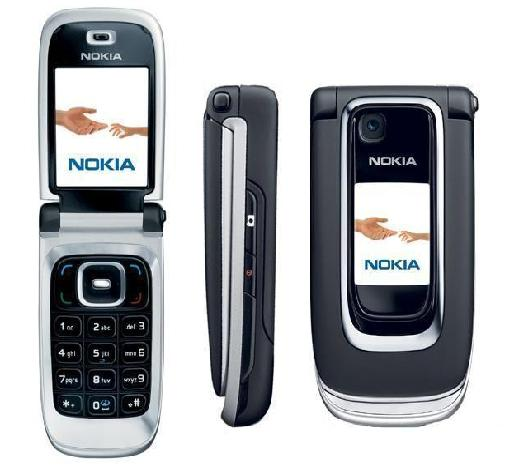
\includegraphics[width=0.6\textwidth]{nokia6131.png}
    \caption{\texttt{Nokia 6131 \acs{NFC}}.}
    \label{fig:nokia6131}
  \end{center}
\end{figure}

Las principales características de este dispositivo móvil son:
\begin{itemize}
\item Similar a la versión \texttt{Nokia 6131} convencional.
\item Peso: 112 gramos.
\item Dimensiones: 92x48x20 mm.
\item Pantalla a color \acs{TFT} de 2.2 pulgadas, con resolución de 240x320 
píxeles.
\item Memoria teléfono: 11 MB.
\item Expansión memoria: microSD (hasta 2 GB).
\item Sistema:
  \begin{itemize}
  \item Configuración \texttt{Java}: \texttt{CLDC 1.1}.
  \item Perfil \texttt{Java}: \texttt{\acs{MIDP} 2.0}.
  \item Versión del \acs{SO}: \texttt{S40}.
  \end{itemize}
\item Conectividad:
  \begin{itemize}
  \item \texttt{Bluetooth 2.0} y \texttt{Bluetooth 2.0 EDR}.
  \item \acs{IrDA}.
  \item \acs{NFC}.
  \end{itemize}
\item Y además:
  \begin{itemize}
  \item Soporta las \acs{API}s \texttt{\acs{JSR}-257} y \texttt{\acs{JSR}-82}.
  \item Soporta la lectura y escritura de los principales formatos de
  etiquetas \acs{RFID}: \texttt{Mifare} (1K, 4K y \emph{Ultralight}),
  \texttt{Topaz}, \texttt{Jewel} y \texttt{Felica}.
  \item Soporta comunicación inalámbrica \acs{P2P}.
  \item Contiene un chip interno de 4K que puede funcionar como una tarjeta
  inteligente \texttt{Mifare} para el alojamiento de datos seguros.
  \end{itemize}
\end{itemize}

El anexo \ref{chap:nokia} contiene las características detalladas de este
dispositivo.

  \subsubsection{Uso de la \acs{API} \texttt{\acs{JSR}-257}}
En la sección \ref{subsec:java} (la tecnología \texttt{Java}) se comentó, que
las \acs{JSR} son \acs{API}s que extienden la funcionalidad estándar de la 
plataforma \texttt{Java}. En este caso, la \texttt{\acs{JSR}-257} va a
proporcionar la funcionalidad necesaria para implementar aplicaciones que
hagan uso de la tecnología \acs{NFC}, como es el caso de la aplicación móvil
del cliente del sistema definido en el presente \acs{PFC}.

A continuación, se va a hacer un repaso de los conceptos básicos que forman
parte del trabajo con etiquetas inteligentes y su implementación a partir
de la \acs{API} \texttt{\acs{JSR}-257}~\cite{bib:jfontecha}:
\begin{itemize}
\item \textbf{Implementación de interfaces}. Para poder hacer uso de las 
funcionalidades \acs{NFC} por medio de \acs{JavaME}
es necesario implementar al menos la interfaz \texttt{TargetListener} en la
clase principal de la aplicación. Esto permitirá la lectura y escritura de
etiquetas una vez iniciada la aplicación.

Si además se desea que, ante el evento de contacto con una etiqueta, sea el 
propio móvil el que inicie la aplicación, se deberá implementar la interfaz
\texttt{NDEFRecordListener}, para provocar el ``autoarranque'' de la aplicación
ante un tipo de etiqueta definido.

Implementar tanto \texttt{TargetListener} como \texttt{NDEFRecordListener},
implica sobreescribir los métodos de dichas interfaces,
\texttt{recordDetected/1} y \texttt{targetDetected/1} respectivamente
(figura \ref{code:extendsNFC}):

\begin{lstlisting}[
  language = Java,
  caption = {Implementación de las interfaces \texttt{TargetListener} y
  \texttt{NDEFRecordListener}.},
  label = code:extednsNFC]
  public class MiMIDLet extends MIDlet implements NDEFRecordListener, TargetListener {
    @override
    void recordDetected(NDEFMessage ndefMessage) { ... }
    @override
    void targetDetected(TargetProperties[] properties) { ... }
  }
\end{lstlisting}

\item \textbf{Descubrimiento de dispositivos y etiquetas}. Para poder leer y 
escribir etiquetas \acs{RFID} con \acs{JavaME}, se necesita realizar un 
descubrimiento previo y añadir el \emph{Listener} correspondiente. De esta 
forma en el constructor del \emph{MIDlet} o nada más iniciar su ejecución, 
podrá realizarse su registro.

Al iniciar el contacto, se registrará el tipo de etiqueta o registro dentro de 
etiqueta que se pretende ``despertar''. El tipo de etiqueta puede
definirse utilizando el formato \acs{MIME} (por ejemplo, \emph{app/mi\_tipo}).
De esta forma, la aplicación estará preparada para leer y escribir etiquetas
con este tipo.

El listado \ref{code:addListener} muestra un ejemplo en el que se añaden
dos \emph{Listener}s:

\begin{lstlisting}[
  language = Java,
  caption = {Se añade un \emph{Listener} para etiquetas \texttt{NDEF} y otro
  para etiquetas \texttt{NDEF} del tipo ``app/mi\_tipo''.},
  label = code:addListener]
  try{
    DiscoveryManager.getInstance().addTargetListener(this, TargetType.NDEF_TAG);
    DiscoveryManager.getInstance().addNDEFRecordListener(this, new NDEFRecordType(NDEFRecordType.MIME, ``app/mi_tipo''));
  } catch(ContactlessException e) { }
\end{lstlisting}

\item \textbf{Conexión y lectura/escritura de datos}. La  interfaz
\texttt{TargetListener} requiere la implementación del método
\texttt{targetDetected}, mediante el cual se definen las acciones a realizar 
cuando se establezca el contacto con una etiqueta \acs{RFID}. El listado
\ref{code:targetDetected} muestra un ejemplo de implementación:

\begin{lstlisting}[
  language = Java,
  caption = {Ejemplo de implementación del método \texttt{targetDetected} en
  la que se realizan varias operaciones.},
  label = code:targetDetected]
  public void targetDetected(TargetProperties[] prop) {
    NDEFTagConnection conn = null;
    //Obtenemos las propiedades de la etiqueta
    TargetProperties target = prop[0];
    try {
      // Obtenemos la url de la etiqueta para ``conectarnos'' con ella
      String url = target.getUrl();
      // Abrimos la conexion y la almacenamos en un objeto NDEFTagConnection
      conn = (NDEFTagConnection)Connector.open(url);
      // Leemos los datos de la etiqueta y los almacenamos en un objeto NDEFMessage
      NDEFMessage message = conn.readNDEF();
      // Obtenemos el numero de registros del mensaje
      NDEFRecord[] records = message.getRecords();
      // Operamos con esos registros y ejecutamos las acciones correspondientes
      // Podemos crear y escribir un nuevo mensaje en la etiqueta de esta forma
      conn.writeNDEF(message);
      //Cerramos la conexion
      conn.close();
    } catch (...) { }
  }
\end{lstlisting}

\item \textbf{Eliminación del \emph{Listener}}. Cuando ya no interese leer o 
escribir etiquetas de un tipo determinado, se eliminará su registro 
correspondiente. Con ello, la aplicación dejará de estar a la escucha de este 
tipo de etiquetas, a menos que se vuelvan a registrar (listado
\ref{code:removeListener}):

\begin{lstlisting}[
  language = Java,
  caption = {Se eliminan los \emph{Listener}s añadidos en el listado
  \ref{code:addListener}.},
  label = code:removeListener]
  try {
    DiscoveryManager.getInstance().removeNDEFRecordListener(this, new
    NDEFRecordType(NDEFRecordType.MIME,``app/mi_tipo''));
    DiscoveryManager.getInstance().removeTargetListener(this, TargetType.NDEF_TAG);
  } catch (...) { }
\end{lstlisting}

\item \textbf{Lectura instantánea de información}. El registro del
\texttt{NDEFRecordListener} permitirá leer datos con el simple
hecho de aproximar el dispositivo móvil a una etiqueta \acs{RFID}, sin 
necesidad de que, la aplicación que hará uso de sus datos, esté en ejecución.
Para ello, debe implementarse el método \emph{RecordDetected}.

El método \texttt{recordDetected} obtiene directamente el objeto de tipo
\texttt{NDEFMessage} que contiene el mensaje de la etiqueta \acs{RFID}
(figura \ref{code:recordDetected}).

\begin{lstlisting}[
  language = Java,
  caption = {El objeto \texttt{peli}, de tipo \texttt{Pelicula}, almacena
  el contenido del registro 0 de la etiqueta, extraído por el lector
  \acs{NFC}.},
  label = code:recordDetected]
  public void recordDetected(NDEFMessage nDEFMessage) {
    // Nos aseguramos que el mensaje contenido en el registro 0 de la etiqueta es de tipo ``app/objeto''
    if (nDEFMessage.getRecord(0).getRecordType().getName().equals(``app/pelicula'')){
      //Obtengo la informacion contenida en ese mensaje y construyo con ella un objeto especifico de mi aplicacion.
      peli = new Pelicula(nDEFMessage.getRecord(0).getPayload());
    }
  }
\end{lstlisting}

Una vez extraída la información de la etiqueta, comenzará la ejecución normal
de la aplicación, teniendo los datos de la etiqueta disponibles para su
tratamiento desde el principio. Sin embargo, para provocar el ``auto-arranque''
de la aplicación, es necesario dar de alta a la misma en el
\emph{Push-Registry} \texttt{Java} del dispositivo móvil.

\item \textbf{El \emph{Push-Registry}}. Es una clase interna \acs{JavaME} que 
permite ejecutar aplicaciones en principio inactivas, ante la respuesta a un 
evento, como puede ser el \emph{timer} de un reloj, la aproximación de una 
etiqueta \acs{RFID} al dispositivo, etc.

Cuando una aplicación define el \emph{Push-Registry} como respuesta a un
evento, este hecho queda registrado en el archivo description de la
aplicacion móvil (archivo con extensión \emph{.jad}).
\end{itemize}

\subsection{Aplicación de la tecnología \texttt{Bluetooth}}
La tecnología ideal para comunicar los dispositivos móviles de los clientes con
los equipos del restaurante sería la tecnología \acs{WiFi}. Desafortunadamente,
el \texttt{Nokia 6131 \acs{NFC}} no cuenta con esta tecnología. Por ello, para
desempeñar tal cometido, se ha seleccionado otra de las tecnologías
inalámbricas que dicho dispositivo si posee, en este caso la tecnología
\emph{Bluetooth}.

  \subsubsection{Introducción de la tecnología \emph{Bluetooth} en el entorno}
La tecnología \emph{Bluetooth} va a facilitar las comunicaciones entre los
dispositivos \acs{NFC} de los clientes y las aplicaciones que forman parte del 
sistema del restaurante.

Las comunicaciones \emph{Bluetooth} entre cliente y restaurante van a seguir 
el esquema \emph{\textbf{cliente-servidor}}. Las aplicaciones del restaurante 
ejecutarán un servidor \emph{Bluetooth} y mantendrán activo un
\textbf{servicio} que será localizable a través de su identificador único, que 
será conocido por el cliente.

Por lo tanto, las conexiones serán iniciadas siempre por parte del cliente, 
cuando alguna de las interacciones \acs{NFC} solicite un servicio del
servidor \emph{Bluetooth} del restaurante. Dependiendo de la interacción, el 
cliente enviará: la solicitud de un pedido, la solicitud de la cuenta o la 
solicitud del ingreso, pago o abandono del local. Todos estos mensajes serán 
enviados irán acompañados de los datos personales (completos o parciales) del 
cliente.

Las respuestas a estas solicitudes serán elaboradas por la correspondiente 
aplicación del restaurante, teniendo en cuenta el estado actual del cliente; y 
se emitirán dentro de la misma conexión. Una vez enviada la respuesta, se
dará por finalizada la comunicación, cerrando la conexión.

Por último, cabe reseñar que, el contar con la tecnología \emph{Bluetooth} va
a ir acompañado de tener que lidiar con sus desventajas (que pudieron verse en 
la sección \ref{subsec:bluetooth}, en el apartado de desventajas). Las que
más pueden afectar a la implementación de la aplicación móvil son las 
siguientes:
\begin{itemize}
\item La velocidad de transmisión es lenta para archivos pesados. En el
caso del \texttt{Nokia 6131 \acs{NFC}}, la versión del \emph{Bluetooth} es
la \texttt{2.0 EDR}, por lo que (según la tabla \ref{tab:btSpeed}, página
\pageref{tab:Speed}), el ancho de banda es de 3 Mbit/s. Afortunadamente, las
transacciones de datos no se antojan muy pesadas.
\item El alcance es bastante limitado. El \emph{Bluetooth} del
\texttt{Nokia 6131 \acs{NFC}} es de \emph{Clase 2}, por lo tanto, según
la tabla \ref{tab:tbClasses} (página \pageref{tab:tbClasses}), el rango
de alcance está en torno a los 25 metros. Dependiendo de la extensión del
restaurante, esto puede suponer un problema.
\item Además, existe una limitación en cuanto a la cantidad de dispositivos 
que pueden estar conectados en una misma red \emph{Bluetooth}. El máximo es de 
8 dispositivos simultáneos. Como se prevé que las comunicaciones van a ser
más o menos rápido, será difícil que se produzcan más de 8 comunicaciones
simultáneas, a no ser que el restaurante tenga un gran aforo y este esté cerca
del completo.
\end{itemize}

  \subsubsection{La comunicación serie virtual}
Como se ha comentado anteriormente, las comunicaciones inalámbricas que se 
produzcan vía \emph{Bluetooth} van consistir en: la emisión de un mensaje de 
solicitud por parte del cliente y la respuesta a este por parte del 
restaurante. Los mensajes no van a tener una gran extensión y van a ser 
enviados en forma de cadena de caracteres\footnote{Dependiendo de la 
complejidad del mensaje, la cadena de caracteres irá o no codificada en 
formato \acs{XML}.}. Por este motivo, una \emph{comunicación en serie virtual} 
puede ser la forma más eficiente para llevar a cabo este
procedimiento\footnote{Si se hubieran tenido que transmitir una gran cantidad
de datos como pueden ser archivos binarios completos, hubiera sido más 
conveniente utilizar otra alternativa, como el protocolo \acs{OBEX} para el 
intercambio de archivos.}.

La \emph{comunicación en serie virtual} funciona de forma similar a la
comunicación en serie (\emph{full-duplex}) entre dos PCs conectados 
mediante una interfaz \texttt{RS-232}. Es decir, también se trata de un
tipo de comunicación bidireccional que permite a dos dispositivos
recibir datos previamente serializados, a la vez que transmitirlos por el
puerto serie.

Los puertos reservados para la comunicación serie cableada son el \texttt{COM1}
y el \texttt{COM2}, mientras que todos los demás \texttt{COMx} (o a partir de
donde se acaban los puertos físicos), pueden ser utilizados para la 
\emph{comunicación en serie virtual}.

En este \acs{PFC}, los puertos virtuales van a ser utilizados por los
dispositivos \emph{Bluetooth} para emular conexiones \texttt{RS-232}
tradicionales.

  \subsubsection{Uso de la \acs{API} \texttt{\acs{JSR}-82}}
Al igual que ocurría con la \texttt{\acs{JSR}-257} para \acs{NFC}, la \acs{API}
\texttt{\acs{JSR}-82} va a proporcionar las clases e interfaces necesarias para
implementar la funcionalidad \emph{Bluetooth} de la aplicación móvil del
cliente.

A continuación, se va a hacer un repaso de las principales clases y métodos
que forman parte del paquete \texttt{javax.bluetooth}, que está orientado a 
las operaciones \emph{Bluetooth} que no utilizan el protocolo \acs{OBEX}.
Como, en este caso, la aplicación del cliente siempre va a ejercer como 
cliente, en el esquema \emph{cliente-servidor}, sólo van a exponerse las
clases orientadas a las comunicaciones cliente \acs{SPP}\footnote{El
\emph{Serial Port Profile} es un perfil \emph{Bluetooth} basado en la
\texttt{\acs{ETSI} 07,10} y en el protocolo \acs{RFCOMM}, que emula
un cable serial para proporcionar un sustituto similar a la interfaz
\texttt{RS-232}, incluyendo sus principales señales de control.}:
\begin{itemize}
\item AAA
\end{itemize}

  \subsubsection{Uso de la biblioteca \texttt{32feet.NET}}
Las aplicaciones del restaurante van a implementarse utilizando el lenguaje
\texttt{Visual C\# .NET}. Por lo tanto, será necesario hacer uso de una 
biblioteca que contenga una implementación en dicho lenguaje de las 
operaciones típicas de un servidor \emph{Bluetooth}. Esta biblioteca es la
\texttt{32feet.NET}

\texttt{32feet.NET} es un proyecto de código fuente compartido que tiene
como objetivo hacer que tecnologías \acs{PAN}, como \texttt{Bluetooth}, 
\acs{IrDA}, etc., sean más fácilmente accesibles desde \texttt{.NET}. Es 
compatible con sistemas de escritorio, móviles o incrustados.
Actualmente, el proyecto se compone de las siguientes tecnologías:
\begin{itemize}
\item \texttt{Bluetooth}.
\item \acs{IrDA}.
\item \acs{OBEX}.
\end{itemize}
El soporte para \emph{Bluetooth} requiere un dispositivo con
\texttt{Microsoft} o con una pila \texttt{Bluetooth Widcomm}. Otros requisitos 
son: \texttt{.NET Compact Framework v2.0} o superior y \texttt{Windows CE .NET 
4.2} o superior; o \texttt{.NET Framework v2.0} o superior para sistemas
operativos \texttt{Windows XP},  \texttt{Windows Vista} o
\texttt{Windows 7}~\cite{bib:32feet}.

A continuación, se va a hacer un rápido repaso de los métodos y operaciones
de la biblioteca \texttt{32feet.NET} que van a intervenir en la creación de un 
servidor \emph{Bluetooth}:
\begin{itemize}
\item AAA
\end{itemize}

\section{Metodología de trabajo}
\label{sec:workingMethodology}
Después de los pasos citados anteriormente se decide, para abordar el
desarrollo del proyecto, optar por una adaptación de la metodología de 
\emph{\textbf{prototipado incremental}}.

  \subsection{Prototipado incremental}
El objetivo de este \acs{PFC} es la creación del prototipo de un sistema.
Según ~\cite{bib:software_engineering}, \emph{``un prototipo puede definirse
como  un modelo parcial ejecutable de un sistema de software''.} Por lo tanto, 
no se pretende crear un producto final comercializable, sino más bien, un
modelo parcial de un sistema que ayude a comprender cómo funcionaría la
implantación de este sistema bajo las condiciones de un entorno real.

Pero, como su nombre indica, se pretende crear un sistema, es decir, un
\emph{``conjunto de cosas que relacionadas entre sí ordenadamente contribuyen 
a determinado objeto''}~\cite{bib:rae}. Por lo que, la creación de este 
prototipo deberá hacerse teniendo en cuenta que está formado por otros 
prototipos más elementales que están relacionados entre sí.

Según ~\cite{bib:software_engineering}, el prototipado incremental \emph{``
se basa en la generación de varios modelos parciales ejecutables del sistema 
antes de proceder a la implementación (durante la especificación y durante el 
diseño) con el fin de evaluar sus características y poder obtener al final el 
sistema implementado.''.}

Cada nuevo ``modelo parcial'' se obtendrá a partir del ``modelo parcial''
anterior (validado por los usuarios y/o los analistas) junto con la
introducción de nuevos elementos funcionales del sistema. Esto se repetirá
hasta tener el sistema completo implementado (figura
\ref{fig:incremental_prototyping}).

\begin{figure}[!h]
  \begin{center}
    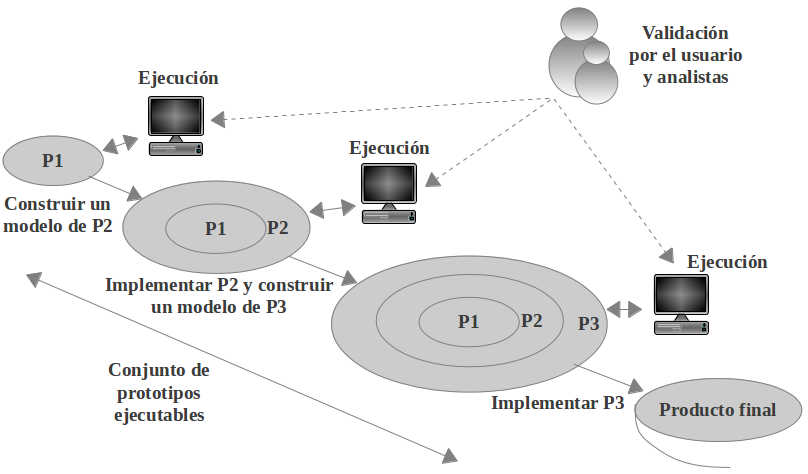
\includegraphics[width=0.9\textwidth]{incremental_prototyping.png}
    \caption{Ciclo de vida del prototipado incremental.}
    \label{fig:incremental_prototyping}
  \end{center}
\end{figure}

Como el sistema está formado por varios prototipos, habrá ``modelos parciales''
en los que estén involucrados varios de estos prototipos y otros en los que
sólo se implementen funcionalidades propias de uno de los prototipos del
sistema.

  \subsection{Estructura general del sistema}
Tras el estudio de campo realizado, las consideraciones del escenario y la
descripción de las principales tecnologías que se van a emplear, se propone
el siguiente escenario (figura \ref{fig:scenario}) como el \emph{escenario
tipo} sobre el cual implementar el sistema.

\begin{figure}[!h]
  \begin{center}
    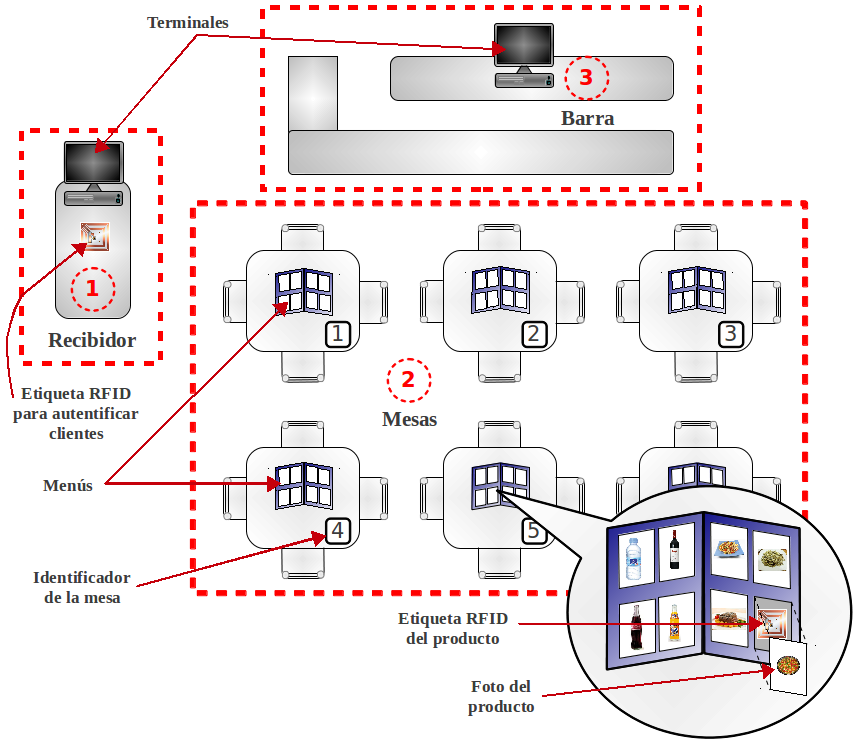
\includegraphics[width=1\textwidth]{scenario.png}
    \caption{Escenario tipo del sistema.}
    \label{fig:scenario}
  \end{center}
\end{figure}

    \subsubsection{El restaurante}
  El restaurante dispondrá de tres zonas claramente definidas:
  \begin{enumerate}
  \item El \textbf{recibidor}. Es la zona por la que se accede al salón del
  restaurante. Estará regentada por un \emph{maître} que, apoyado por un 
  terminal, registrará la entrada y salida de clientes y la asignación de 
  mesas. Además, el \emph{maître} también se encargará de gestionar los cobros 
  mediante \acs{NFC}.
  \item Las \textbf{mesas}. Cada mesa tendrá un identificador único que la
  diferencie de las demás mesas. Este identificador servirá para poder
  asociar al cliente registrado con la mesa que está ocupando. Cada mesa
  contará con una carta de productos compuesta por varias etiquetas
  \acs{RFID}. Cada etiqueta contendrá la información de un producto. Esto 
  permitirá al cliente elaborar la lista de productos para un pedido
  mediante su dispositivo móvil \acs{NFC}.
  \item La \textbf{barra}. Es la zona donde se reciben los pedidos. Algunos
  podrán ser atendidos sobre la marcha por los camareros y otros necesitarán
  ser elaborados antes por los cocineros. Todos los pedidos recibidos serán
  registrados en un terminal, de manera que se vaya generando una lista de
  pedidos por cada mesa. Esto ayudará a la gestión del estado de dichos 
  pedidos y a la facturación (en conjunto) de los mismos.
  \end{enumerate}

  Tanto el terminal del recibidor como el terminal de la barra dispondrán
  de un punto de conexión \emph{Bluetooth}, para posibilitar la comunicación
  con el dispositivo móvil de los clientes.

  Por otro lado, uno de los terminales citados u otro terminal distinto (que
  no tiene porqué estar en el mismo establecimiento) se encargará de hospedar
  al \textbf{servicio web}, que es la entidad a la que recurren los otros
  terminales para actualizar sus datos.

  Con la \textbf{base de datos} ocurre lo mismo. Puede encontrarse en uno de
  los terminales del restaurante, en el mismo terminal que el servicio web o
  en un terminal distinto. Se encargará de garantizar la persistencia de los
  datos generados por el sistema.

%  La figura \ref{fig:structure} muestra la estructura general del sistema.

%  \begin{figure}[!h]
%    \begin{center}
%      \includegraphics[width=0.8\textwidth]{structure.png}
%      \caption{Estructura general del sistema.}
%      \label{fig:structure}
%    \end{center}
%  \end{figure}

    \subsubsection{Los clientes}
    \label{subsubsec:clients}
  Habrá dos tipos de clientes:
  \begin{enumerate}
  \item \emph{\textbf{Clientes \acs{NFC}}}. Son potenciales \emph{clientes
  \acs{NFC}} los clientes que tienen un móvil con la tecnología \acs{NFC} y
  \emph{Bluetooth}. La tecnología \acs{NFC} les permitirá realizar acciones
  como: comunicar su llegada o su salida, pagar o elaborar una lista de
  productos para un pedido; con el simple gesto de tocar unas u otras
  etiquetas \acs{RFID}. El \emph{Bluetooth} por su parte, permitirá la
  comunicación entre el dispositivo del cliente y los terminales del
  restaurante para, por ejemplo: mandar sus datos personales, recibir
  recomendaciones, enviar pedidos o recibir el resumen de su factura.
  \item \emph{\textbf{Clientes normales}}. Los clientes que no disponen
  de un dispositivo móvil con las características de los \emph{clientes
  \acs{NFC}} o que simplemente no hacen uso de él. Su conducta para con
  el restaurante será la misma que la que se sigue comunmente en este tipo
  de establecimientos: solicita una mesa al \emph{maître}, se sienta,
  pide al camarero lo que desea tomar, se lo sirven, lo consume, solicita
  la cuenta, paga y se va. Este tipo de clientes no podrá recibir
  recomendaciones y no disfrutará de los descuentos que sí se le aplican
  a los \emph{clientes \acs{NFC}}.
  \end{enumerate}

  \subsection{Fases del prototipo}
Como se dijo anteriormente, el prototipo del sistema se construirá de forma
incremental a partir de varias iteraciones en las que se irán añadiendo
nuevas funcionalidades al sistema elemental (de la primera iteración). Las
iteraciones propuestas para el desarrollo del sistema son las siguientes:
\begin{enumerate}
\item Prototipo inicial de los servicios web y la base de datos.
\item Prototipo inicial de la aplicación del \emph{recibidor} y conexión con 
los servicios web.
\item Prototipo inicial de la aplicación de la \emph{barra} y conexión con los 
servicios web.
\item Prototipo inicial de la aplicación móvil.
\item Conexiones \emph{Bluetooth} entre el prototipo del móvil y el del
\emph{recibidor}.
\item Conexiones \emph{Bluetooth} entre el prototipo del móvil y el de la
\emph{barra}.
\item Sistema recomendador.
\end{enumerate}

\section{Herramientas}
En esta sección se citan las herramientas que han sido utilizadas para el 
desarrollo de este \acs{PFC}.

  \subsection{Diagramas \acs{UML}}
  Para cubrir la fase de análisis de requisitos y el diseño de cada una de las
  iteraciones propuestas se ha echado mano del \emph{\textbf{Visual Paradigm
  for \acs{UML}}}, que es una herramienta \emph{case} de especificaciones
  \acs{UML}, desarrollado por la empresa \emph{Visual Paradigm International}.

%%%%%%%%
%%%%%%%% de momento sólo diagramas de casos de uso, de secuencia y de clases
  Con este programa se han realizado los diagramas de casos de uso, los de
  clases, los de despliegue, los de comunicación y los de secuencia. Es decir,
  todos los diagramas que definen la forma en la que está estructurado el
  sistema y la forma en que se comporta.

  La versión utilizada ha sido la \emph{8.3} de la \emph{Community Edition} y
  ha sido necesario solicitar una licencia gratuita, para uso \emph{no 
  comercial}.

  \subsection{Lenguajes de programación}
  El código de los distintos elementos que forman parte del sistema ha sido
  implementado utilizando los siguientes lenguajes de programación:

  \begin{itemize} 
  \item \textbf{C\#}.
  Es un lenguaje de programación \acs{OO} (Orientada a Objetos) desarrollado y
  estandarizado por \emph{Microsoft} como parte de su plataforma \emph{.NET}.

  Con este lenguaje se ha desarrollado la aplicación del \emph{recibidor} y
  la aplicación de la \emph{barra}.

  Además, se ha utilizado la librería externa \emph{InTheHand.Net}, que
  posibilita las conexiones \emph{Bluetooth} de las aplicaciones implementadas
  en \emph{C\#} con los dispositivos móviles.

  \item \textbf{ASP.NET}.
  En realidad \emph{ASP.NET} no puede 
  considerarse un lenguaje de programación, más bien es un \emph{framework} 
  que se utiliza para la construcción de sitios web dinámicos, aplicaciones 
  web o servicios web \acs{XML}. \emph{ASP.NET} está construido sobre el
  \emph{Common Language Runtime}, lo que permite a los programadores escribir 
  código \emph{ASP.NET} utilizando cualquier lenguaje admitido por el
  \emph{framework} de \emph{.NET}, como por ejemplo, el propio \emph{C\#}.

  Los servicios web han sido implementados utilizando el \emph{framework}
  \emph{ASP.NET}.

  Además, para poder acceder a la base de datos, se ha utilizado una librería
  externa a \emph{C\#} llamada \emph{MySql.Data}.

  \item \textbf{SQL}.
  \acs{SQL} es un lenguaje declarativo de acceso a bases de
  datos relacionales que permite especificar distintos tipos de operaciones
  sobre estas.

  En este caso la base de datos a la que se accede está montada sobre un
  \acs{SGBD} \emph{MySQL}. Esta base de datos almacena todos los datos de
  interés con los que trabajan las dos aplicaciones del restaurante
  (\emph{recibidor} y \emph{barra}).

  \item \textbf{Java Micro Edition}.
  Es una especificación de un subconjunto de la
  plataforma \emph{Java} orientada a proveer una colección certificada de
  \acs{API}s de desarrollo de software para dispositivos con recursos
  restringidos, como son los dispositivos móviles.

  \acs{JavaME} fue desarrollado mediante el Java Community Process bajo la 
  especificación \texttt{\acs{JSR}-68}. La evolución de la plataforma ha 
  propiciado el abandono de las \emph{Java Specification Request} (peticiones  
  de especificación para \texttt{Java}) en favor de \acs{JSR}s separadas para  
  las distintas versiones de \acs{JavaME}.

  Por ejemplo, para el desarrollo de la aplicación móvil se han utilizado
  principalmente dos \acs{JSR}s:
    \begin{itemize}
    \item \textbf{\acs{JSR}-82}. Que implementa las funcionalidades
    propias de las comunicaciones vía \emph{Bluetooth} entre dispositivos.
    \item \textbf{\acs{JSR}-257}. Que implementa las funcionalidades propias
    de las comunicaciones \acs{NFC}.
    \end{itemize}

  Además de estas, también se ha hecho uso de la librería
  \texttt{kxml2-min-2.3.0} que permite construir y recorrer documentos o 
  cadenas expresados en \acs{XML}.

  \item \textbf{XML}.
  Es un lenguaje de marcas desarrollado por el
  \emph{World Wide Web Consortium} (\acs{W3C}). Permite definir la gramática de
  lenguajes específicos para estructurar documentos grandes. A diferencia de
  otros lenguajes, \acs{XML} da soporte a bases de datos, siendo útil cuando
  varias aplicaciones se deben comunicar entre sí o integrar información.

  En este caso, se utiliza \acs{XML} para mandar información estructurada 
  entre las aplicaciones del restaurante y los servicios web (a través de la
  red) y entre los dispositivos móviles y las aplicaciones del restaurante 
  (esta vez vía \emph{Bluetooth}). El anexo \ref{chap:xmls} muestra los 
  distintos tipos de elementos que han sido definidos utilizando \acs{XML}.
  \end{itemize}

  \subsection{Aplicaciones de desarrollo}
  Para implementar las distintas aplicaciones que conforman el sistema se
  ha hecho uso de las siguientes herramientas de desarrollo:
  
  \begin{itemize}
    \item \textbf{Microsoft Visual Studio 2010}.
    Es un entorno de desarrollo integrado (\acs{IDE}) para sistemas operativos
    \emph{Windows}. Soporta lenguajes de programación como \emph{Visual C++},
    \emph{Visual C\#}, \emph{Visual J\#}, \emph{Visual Basic .NET} y
    entornos de desarrollo web como \emph{ASP.NET}, aunque actualmente
    se han desarrollado extensiones para muchos otros.

    Este \acs{IDE} se ha utilizado para desarrollar la aplicación del
    \emph{recibidor}, la aplicación de la \emph{barra} y los servicios web.
    
    \item \textbf{Netbeans IDE 7.0.1}.
    Es un \acs{IDE} libre que no tiene restricciones de uso, concebido 
    originalmente por \emph{Sun MicroSystems} para el desarrollo de proyectos
    en lenguaje \emph{Java}, aunque actualmente existe un gran número de 
    módulos que extienden su funcionalidad.

    Este \acs{IDE} se ha usado para crear la aplicación del dispositivo móvil.
    Para su desarrollo ha sido necesario incluir el módulo \emph{Mobility 
    Pack}, que permite desarrollar aplicaciones en \acs{JavaME}.

    \item \textbf{SDK Nokia 6131 NFC}. 
    Es un kit de desarrollo software (\acs{SDK}) que proporciona una serie
    de \acs{API}s de desarrollo de aplicaciones para el dispositivo móvil
    \emph{Nokia 6131 \acs{NFC}} y, junto al \acs{IDE} \emph{Netbeans},
    permite emular las funcionalidades implementadas sin necesidad de
    cargarlas en un dispositivo móvil real.
    
    \item \textbf{phpMyAdmin 3.4.10.1}.
    Es una herramienta escrita en \emph{PHP} que permite administrar bases
    de datos \emph{MySQL} a través del navegador.

    Ha sido la herramienta utilizada para crear y editar las tablas que
    forman parte de la base de datos del sistema y, en general, la herramienta
    utilizada para administrar los contenidos de dichas tablas.

    La base de datos utilizada para probar el sistema se encuentra en la
    dirección: \url{161.67.140.37:3500/}.
    %%%%%%%%%%%%%%%%%%%%%%%%%%%%%%%%%%%%%
    %%%%%% ¿Poner también usuario y contraseña para acceder a las BBDD?
    Los servicios web por su parte
    pueden ser accedidos a través de la dirección:
    \url{161.67.140.37:3500/ServicioMobiCarta/Services.asmx}. Ambas
    direcciones pertenecen a uno de los serviciores del grupo \acs{MAmI}.
  \end{itemize}

  \subsection{Repositorio de datos}
  Para un mejor mantenimiento y accesibilidad de la información generada
  durante el desarrollo del \acs{PFC}, se ha optado por almacenar dicha
  información en los repositorios de \emph{Google Code}.

  \emph{Google Code} es una herramienta de \emph{Google} para desarrolladores 
  interesados en el desarrollo de proyectos \emph{open-source}. \emph{Google}
  cede su espacio con la única condición de que la información del proyecto
  sea accesible a todo el mundo.

  La dirección de este \acs{PFC} es la siguiente:\\
  \url{http://code.google.com/p/restaurant-management-using-nfc/}.

  \subsection{Control de versiones}
  \emph{``Se llama control de versiones a la gestión de los diversos cambios 
  que se realizan sobre los elementos de algún producto o una configuración 
  del mismo. Una versión, revisión o edición de un producto, es el estado en 
  el que se encuentra dicho producto en un momento dado de su desarrollo o 
  modificación.''}~\cite{bib:wiki}.
  
  En este caso, como se trabaja con un sistema complejo, formado por varios 
  elementos, cada elemento va generando información en cada etapa de 
  desarrollo y en cada etapa de desarrollo se trabaja con varios archivos; es 
  del todo recomendable registrar en un control de versiones las modificaciones
  que se van realizando en cada uno de los archivos. Esto posibilita llevar
  un seguimiento del cuándo, el dónde y el porqué de cada uno de los cambios;
  y permite volver a estados (o revisiones) anteriores. Además, en colaboración
  con el repositorio de datos, permite tener actualizado el estado de 
  todos los archivos del proyecto aunque el desarrollo se esté realizando en 
  distintas máquinas.

  El sistema de control de versiones (\acs{SVC}) utilizado en este \acs{PFC}
  ha sido \emph{Mercurial}. \emph{Mercurial} es un \acs{SVC} con 
  licencia \emph{\acs{GPL} v2}, multiplataforma, escrito en \emph{Python}.

  Para sistemas \emph{Linux} es habitual utilizar \emph{Mercurial} desde el
  terminal. En sistemas \emph{Windows}, por el contrario, es más común utilizar
  herramientas gráficas que faciliten la ejecución de las principales tareas
  de este \acs{SVC}. En este caso, se han utilizado las siguientes herramientas
  disponibles todas ellas en la página de \emph{Mercurial}
  (\url{http://mercurial.selenic.com/}):
  \begin{itemize}
    \item \emph{\textbf{TortoiseHg 2.2.2}}. Es un conjunto de herramientas 
    gráficas y extensiones de la \emph{shell} para \emph{Mercurial}.
    \item \emph{\textbf{VisualHg}}. Es una extensión para \emph{Visual Studio}
    que permite utilizar la funcionalidad de \emph{Mercurial} sobre los
    archivos de la solución actual.
    \item \emph{Extensión de Mercurial para Netbeans}. Como ocurre con
    \emph{Visual Studio}, también existe una extensión que permite utilizar
    las funcionalidades de \emph{Mercurial} sobre los archivos de los 
    proyectos cargados.
  \end{itemize}

  \subsection{Edición de imagen y gráficos vectoriales}
  Para la elaboración de los iconos y otras imágenes de las aplicaciones, así
  como para la edición de las imágenes del presente documento, se han utilizado
  los siguientes programas:
  \begin{description}
  \item[Gimp 2.6.] \emph{Gimp} o (\emph{\acs{GNU} Image Manipulation Program})
  es un programa de edición de imágenes digitales en forma de mapas de bits.
  Forma parte del proyecto \acs{GNU} y está disponible bajo la licencia
  \acs{GPL}.
  \item[Inkscape 0.48.3.1.] \emph{Inkscape} es un editor de gráficos 
  vectoriales en formato \acs{SVG}. Las características \acs{SVG} soportadas
  incluyen formas básicas, trayectorias, texto, canal alfa, transformaciones,
  gradientes, edición de nodos, exportaciones a \acs{PNG}, agrupación de
  elementos, etc. Al igual que \emph{Gimp}, \emph{Inkscape} también es un
  programa multiplataforma disponible bajo la licencia \acs{GPL}.
  \end{description}

  \subsection{Documentación}
  Para la composición de este documento se ha utilizado el sistema de
  composición de textos \LaTeX. \LaTeX es un sistema de composición muy
  adecuado para realizar artículos académicos, tesis y libros técnicos, dado
  que la calidad tipográfica de los documentos realizados es comparable a la
  de una editorial científica de primera línea\cite{bib:LaTeX}. \LaTeX es
  software libre bajo licencia \acs{LPPL}.

  Además, se ha utilizado como tipo de documento la clase \emph{arco-pfc}, que
  es una clase elaborada por el \emph{grupo \acs{ARCO}}\footnote{Grupo de
  investigación de la \acs{UCLM} que tiene como objetivo el diseño de
  sistemas complejos con componentes tanto hardware como software, haciendo
  especial énfasis en aspectos como la utilización de recursos, prestaciones
  y comunicaciones, y su aplicación al desarrollo de servicios avanzados en
  áreas tales como la computación distribuida, inteligencia ambiental, redes
  de sencites, \dots~\cite{bib:ARCO}} para la elaboración de \acs{PFC}s y
  \acs{TFG}s y que sigue el formato especificado por la \acs{ESI} de Ciudad 
  Real. \emph{arco-pfc} es un proyecto libre alojado en la web
  \url{https://bitbucket.org/arco_group/arco-pfc}.

  \subsection{Herramientas hardware}
  Las aplicaciones que forman parte del sistema han sido desarrolladas en
  varios ordenadores personales sobre sistemas operativos como: \emph{Windows
  XP SP3}, \emph{Windows 7} y \emph{Ubuntu 12.04}.

  Fuera de esto, para realizar las pruebas reales del sistema, se han utilizado
  los siguientes medios hardware:
  \begin{itemize}
  \item \textbf{\emph{Nokia 6131 \acs{NFC}}}. Dispositivo donde se ejecuta
  la aplicación móvil. Dispone de lector \acs{NFC} y conexión \emph{Bluetooth}.
  \item \textbf{\emph{Etiquetas \acs{RFID}}}. Tienen 1KB de capacidad. 
  Almacenan sobre mensajes \acs{NDEF} la información de los productos de la 
  carta y de otras operaciones disponibles para el cliente.
  \item \textbf{Monitor táctil}. La aplicación del \emph{recibidor} y la 
  aplicación de la \emph{barra} están enfocadas a la interacción táctil. Por 
  ello es conveniente realizar las pruebas sobre un dispositivo que aproveche 
  esta característica. %%%%%%%%%%%%%%%%%%%%%%%%%%%%%%%%%%
  %%%%%% ¿Qué características tiene el monitor táctil? Modelo, dimensiones, etc.
  \end{itemize}

% Local Variables:
%   coding: utf-8
%   mode: latex
%   mode: flyspell
%   ispell-local-dictionary: "castellano8"
% End:
